The ProtoDUNE-SP (NP04) experiment will be housed in the EHN1 building at CERN. The detector is situated at the end of the H4 beamline in the newly constructed extension of EHN1. The H4 beamline is designed in such a way that it can be configured to deliver either a hadron beam or a pure electron beam to the experiment. To produce particles in the momentum range of interest, the secondary beam from the T2 primary target is sent onto a secondary target to generate a tertiary beam. Particles in the tertiary beam are momentum- and charge-selected and transported down the H4 beamline extension to the detector. 
In principle, the H4 beamline can operate in parallel with the H2 beamline, which will intercept the ProtoDUNE-DP (NP02) detector, installed in the same building. In this Chapter, we discuss the beam requirements, H4 beamline design and instrumentations, and DAQ/trigger.  
%The beamline layout is described and illustrated in Section~\ref{sec:h4beamline}. % minimize interference between the two ProtoDUNE experiments.

%%%%%%%%%%%%%%%%%%%%%%%%%%%%%%%%%%%%%%%%%%%%%%
\section{Beam requirements}
\label{sec:beamrequirements}

The CERN test beam results from ProtoDUNE-SP will be used to evaluate the detector performance,  understand the various physics systematic effects, and provide data for event reconstruction studies that are representative of neutrino interactions. 
The parameters defining the test beam are primarily driven by the requirement that these test beam results be directly applicable to DUNE's future large underground single-phase detector module(s) with minimal extrapolation.
The expected momentum distributions for secondary particles from neutrino interactions in the far detector has a large spread that ranges from a few hundred MeV/c to a few GeV/c.
To match the charged-particle spectrum and topologies that are expected in the DUNE far detector, the beam thus must span a broad range of particle momenta, be composed of electrons, muons, and hadrons, and charge-selected. 
Based on the feedback and constraints from the CERN accelerator group, the beamline design has been developed to allow the transport of beam particles from about 0.5~GeV/c up to 7~GeV/c. 

The maximum electron drift time in the ProtoDUNE-SP TPC is about 2.25~ms. In order
to keep the  pile-up of beam particles in the TPC event frame at the percent level, the planned
beam particle rate should be below 100 Hz.  
The ProtoDUNE-SP TPC has two drift volumes separated by a cathode plane. It is desirable to aim the particle beam such
that a large fraction of the lower-energy hadronic showers are 
contained in one drift volume.
As shown in Figure~\ref{fig:beamwindow_loc}, multiple beam injection points have been considered. The larger angle (beam \# 3) w.r.t. the APA plane, which corresponds to about 13$^\circ$ is the preferred beam injection point.
Due to engineering and safety considerations, only beam \#3 will
be fully instrumented with the beam window system as described in
Sections~\ref{subsec:fc-beamplug} and ~\ref{subsec:beamwindow}.
%The angles of the beam, with respect to the APA plane
%are 3$^\circ$ (beam \#1), 8$^\circ$ (beam \#2), and 12$^\circ$ (beam \#3). 
The remaining two beam positions will have partial installation of the beam window system. With this
configuration, beam \#3 is the primary beam %where 
with which most of the physics
data will be taken.
\begin{cdrfigure}[Beam window locations]{beamwindow_loc}{Planned beam window locations.}
  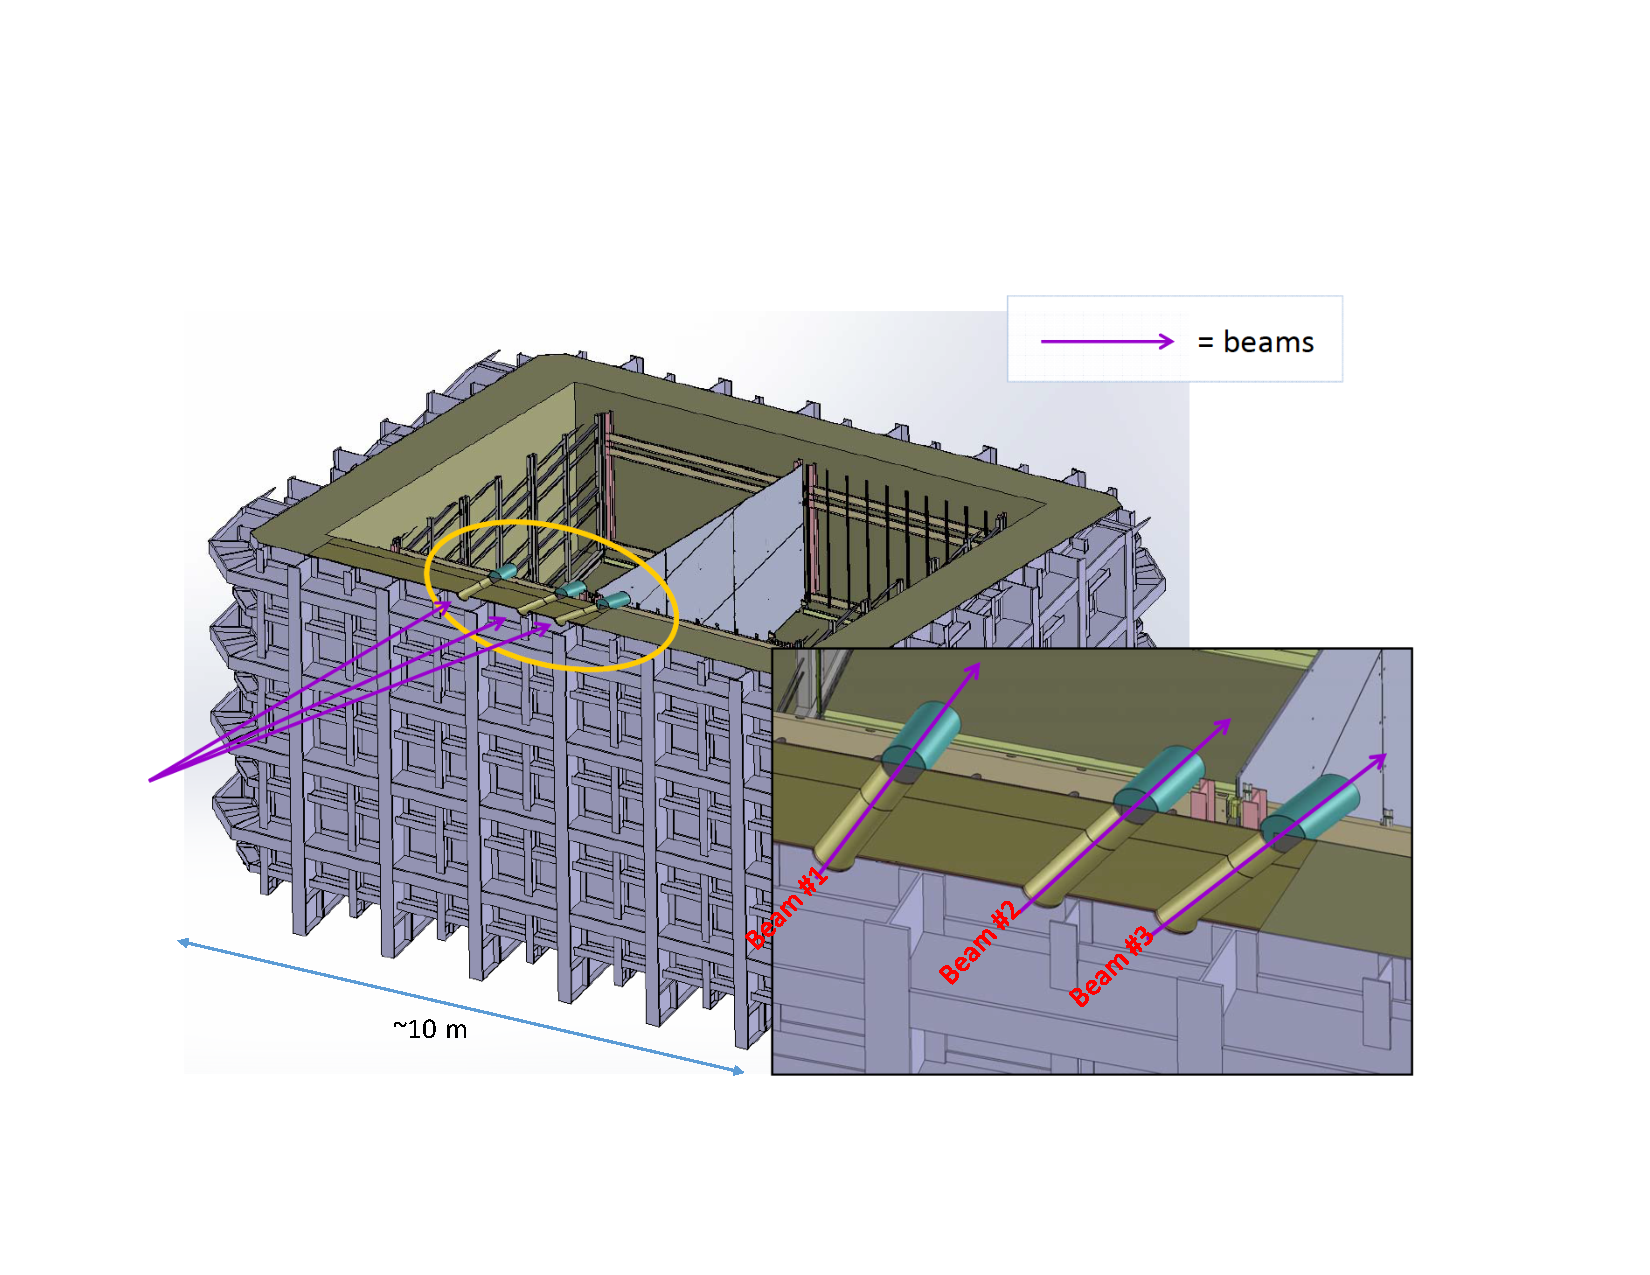
\includegraphics[width=0.9\textwidth]{beamwindow_locations.pdf}
\end{cdrfigure}
\fixme{ Although explained in the text, this figure with three equal beam penetrations/plugs is misleading, should be modified}
A summary of the beam requirements is shown in Table~\ref{tab:beamspecs}.
\begin{cdrtable}[Particle beam requirement]{ll}{beamspecs}{Particle beam requirements. }
%\textbf{Parameter } & \textbf{Requirements}  \\ \hline
 Parameter & Requirements \\ \toprowrule
  Particle Types        & $e^\pm,\mu^\pm,\pi^\pm$,$K$,$p$  \\ \colhline
  Momentum Range   & $\approx$ 1 - 7 GeV/$c$ (hadron beam)\\
                   & 0.5 - 7 GeV/$c$ (electron beam) \\ \colhline
  Momentum spread   & $\Delta p/p   \le 5$ \% (nominal collimator opening) \\ \colhline
  Transverse Beam Size   & RMS(x,y) $\approx$ 1 cm  \\
  & (At the entrance face of the LAr cryostat) \\ \colhline
%  Beam Divergence & tbd   \\ \colhline
  Beam Entrance Position & Beam \# 3 (Figure~\ref{fig:beamwindow_loc})    \\ \colhline
  Rates & 25 - 100 Hz (adjustable)     \\ \colhline
\end{cdrtable}

%\fixme{we should have beam divergence estimates from H2 and H4 simulation files Paola: again, the data from Nikos are a result,  NOT a requirement. If the physics or measurements group do have a requirement, please provide one! I took the line out, waiting for input.}
%\fixme{rate: max of 100 Hx; nominal 25Hz with goal to achieve 50 Hz (see CERN workshop)}
